\documentclass{article}
\usepackage{pgfplots}
\pgfplotsset{compat=1.18}

\begin{document}

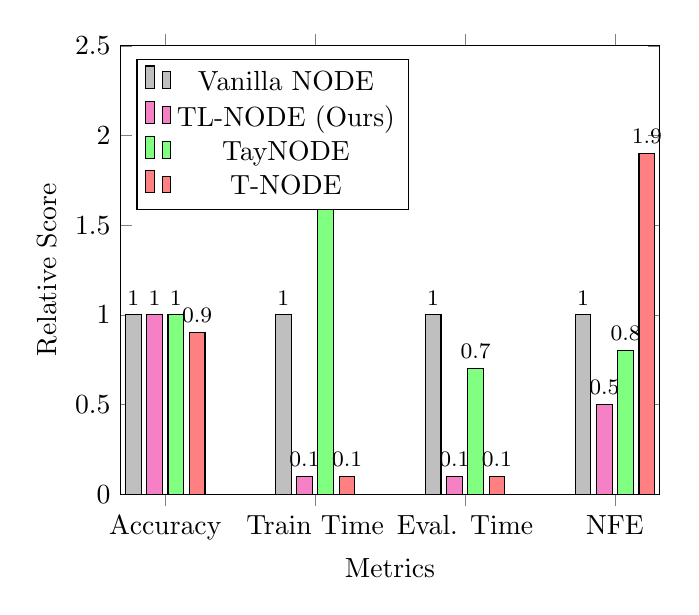
\begin{tikzpicture}
    \begin{axis}[
        ybar,
        bar width=0.2cm,
        ymin=0,
        ymax=2.5,
        ylabel={Relative Score},
        xlabel={Metrics},
        xtick=data,
        xticklabels={Accuracy, Train Time, Eval. Time, NFE},
        legend pos=north west,
        symbolic x coords={Accuracy, Train Time, Eval. Time, NFE},
        nodes near coords,
        every node near coord/.append style={font=\footnotesize},
        ]
        \addplot[fill=gray!50] coordinates {(Accuracy, 1) (Train Time, 1) (Eval. Time, 1) (NFE, 1)};
        \addplot[fill=magenta!50] coordinates {(Accuracy, 1) (Train Time, 0.1) (Eval. Time, 0.1) (NFE, 0.5)};
        \addplot[fill=green!50] coordinates {(Accuracy, 1) (Train Time, 2) (Eval. Time, 0.7) (NFE, 0.8)};
        \addplot[fill=red!50] coordinates {(Accuracy, 0.9) (Train Time, 0.1) (Eval. Time, 0.1) (NFE, 1.9)};
        
        \legend{Vanilla NODE, TL-NODE (Ours), TayNODE, T-NODE}
    \end{axis}
\end{tikzpicture}

\end{document}